\documentclass[lang=cn,11pt,a4paper,cite=authornum]{paper}

\title{操作系统 实验:内存管理 \\ 实验报告}
\author{毛子恒 \\ 2019211397}
\institute{北京邮电大学\ 计算机学院}

\date{\zhtoday}

% 本文档命令
\nocite{*}

\begin{document}

\maketitle

\section{概览}

\subsection{实验目的}

基于openEuler操作系统,通过模拟实现按需调页式存储管理的几种基本页面置换算法,了解虚拟存储技术的特点,掌握虚拟存储按需调页式存储管理中几种基本页面置换算法的基本思想和实现过程,并比较它们的效率。

\subsection{实验内容}

首先用\mintinline{text}{srand()}和\mintinline{text}{rand()}函数定义和产生指令地址序列,然后将指令地址序列变换成相应的页地址流。

设计以下三种算法:

\begin{itemize}
    \item 最优置换算法(Optimal)
    \item 最近最少使用(Least Recently Used)
    \item 先进先出法(Fisrt In First Out) 
\end{itemize}

其中,缺页率=页面失效次数/页地址流长度

要求:分析在同样的内存访问串上执行,分配的物理内存块数量和缺页率之间的关系; 并在同样情况下,对不同置换算法的缺页率比较。

\subsection{实验环境}

\begin{itemize}
    \item openEuler 20.03 64bit with ARM
    \item gcc version 7.3.0
    \item vim 8.1
\end{itemize}

\section{实验设计}

\subsection{随机数生成}

通过随机数产生一个内存地址,共300个地址,地址按下述原则生成∶

\begin{itemize}
    \item 70\%的指令是顺序执行的。
    \item 10\%的指令是均匀分布在前地址部分。
    \item 20\%的指令是均匀分布在后地址部分。
\end{itemize}

具体生成规则为:

\begin{enumerate}
    \item 从地址0开始。
    \item 若当前指令地址为$m$,按上面的概率确定要执行的下一条指令地址,分别为顺序、在前和在后:
    \begin{itemize}
        \item 顺序执行:地址为$(m+1)\bmod 300$的指令。
        \item 在前地址:$[0,m-1]$中依前面说明的概率随机选取地址。
        \item 在后地址:$[m+1, 299]$中依前面说明的概率随机选取地址。
    \end{itemize}
    \item 重复3直至生成$300$个指令地址。
\end{enumerate}

假设每个页面可以存放15条指令,将指令地址映射到页面,生成内存访问串。

\subsection{页面置换算法设计}

\paragraph{LRU置换算法}

采用计数器记录页表中每个条目的使用时间,每次引用一个页或者置换一个页时,将它对应的计数器设为0,将其它页的计数器自增1。

算法的主要部分如下:

\begin{code}
\begin{minted}{C}
for (int i = 0; i < ins_num; ++i)
{
    int max_index = 0, max_count = 0;
    bool hit = false;
    for (int j = 0; j < frame_num; ++j)
    {
        if (frame[j] == address[i])
        {
            hit = true;
            max_index = j;
            break;
        }
        if (frame[j] == -1) // 当前帧为空
        {
            max_index = j;
            break;
        }
        if (count[j] > max_count)
        {
            max_count = count[j];
            max_index = j;
        }
    }
    for (int i = 0; i < frame_num; ++i)
        count[i]++;
    count[max_index] = 0;
    if (!hit)
    {
        tot_miss++;
        frame[max_index] = address[i];
    }
}
\end{minted}
\end{code}

\paragraph{FIFO置换算法}

采用一个指针指向当前队列的队首,每次置换时替换队首的页,并且将指针自增1。

算法的主要部分如下:

\begin{code}
\begin{minted}{C}
for (int i = 0; i < ins_num; ++i)
{
    bool hit = false;
    for (int j = 0; j < frame_num; ++j)
    {
        if (frame[j] == address[i])
        {
            hit = true;
            break;
        }
    }
    if (!hit)
    {
        tot_miss++;
        frame[ptr] = address[i];
        ptr = (ptr + 1) % frame_num;
    }
}
\end{minted}
\end{code}

\paragraph{最优置换算法}

首先对内存访问串进行预处理,计算出$next[i,j]$表示第$i$个内存访问后第一个访问页$j$的位置,每次置换页时,从页表中挑选$next$最大的页即可。

算法的主要部分如下:

\begin{code}
\begin{minted}{C}
for (int i = ins_num - 2; ~i; --i)
    for (int j = 0; j < ins_num; ++j)
    {
        if (address[i + 1] == j)
            next[i][j] = i + 1;
        else
            next[i][j] = next[i + 1][j];
    }
for (int i = 0; i < ins_num; ++i)
{
    int max_index = 0, max_count = 0;
    bool hit = false;
    for (int j = 0; j < frame_num; ++j)
    {
        if (frame[j] == address[i])
        {
            hit = true;
            break;
        }
        if (frame[j] == -1)
        {
            max_index = j;
            break;
        }
        if (next[i][frame[j]] > max_count)
        {
            max_count = next[i][frame[j]];
            max_index = j;
        }
    }
    if (!hit)
    {
        tot_miss++;
        frame[max_index] = address[i];
    }
}
\end{minted}
\end{code}

\subsection{分析}

对于上述的数据规模,假定页表大小为5,随机生成100条数据,得到如\figref{fig:1}的结果。

\begin{figure}[htbp]

    \centering
    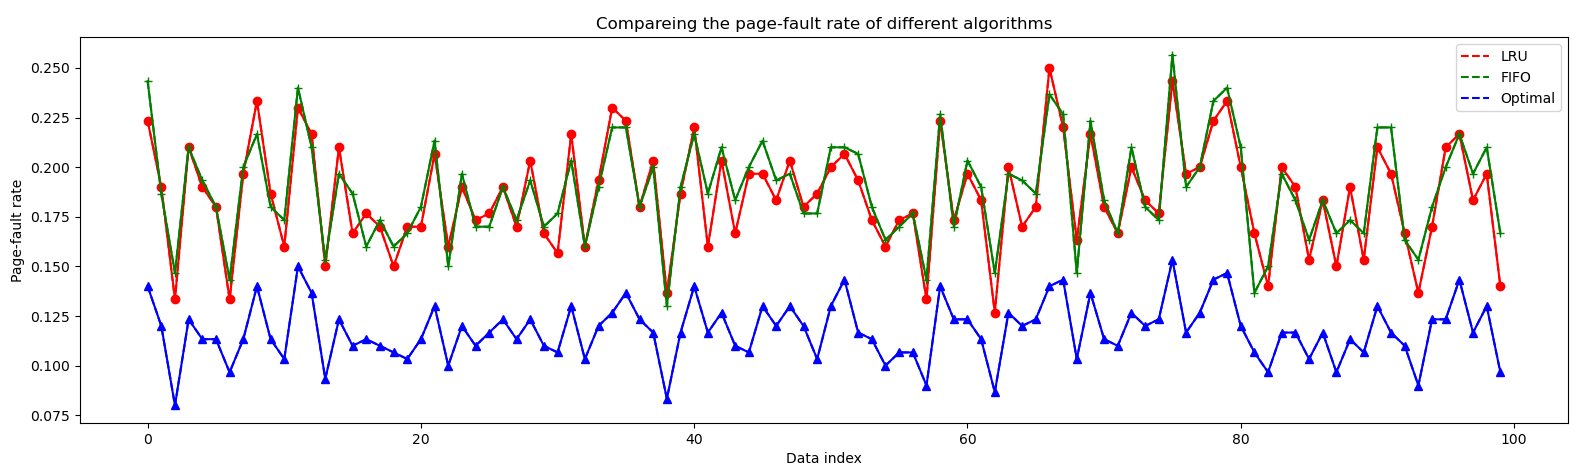
\includegraphics[width=\textwidth]{./images/Figure_1.png}
    \caption{\label{fig:1}}

\end{figure}

可以发现最优置换算法的缺页错误率明显低于其他两种,FIFO算法和LRU算法的缺页错误率接近,但是大部分情况下LRU的缺页错误率更低,LRU算法没有表现出比FIFO算法优更多的性能,推测是由于生成的数据局部性不够强导致。

对于以下数据,在不同页表大小下测试三种算法的缺页错误率:

\begin{code}
\begin{minted}{text}
0 0 18 18 18 18 18 18 19 19 19 19 19 19 19 19 0 0 0 0 0 0 0 0 0 0 0 0 0 0 0 0 1 1 1 1 1 1 1 1 1 1 1 1 0 0 0 0 4 0 0 0 18 18 18 18 18 9 9 9 9 10 10 10 10 10 10 10 10 10 5 6 6 1 1 1 1 10 11 11 11 11 11 11 11 11 6 6 6 6 1 1 0 0 0 4 4 0 0 0 0 10 10 4 4 4 4 1 1 1 1 1 1 18 19 19 19 19 19 19 0 0 0 0 0 0 9 9 9 14 14 15 15 15 15 15 16 16 16 16 16 16 16 16 16 14 14 14 0 0 0 0 0 15 15 16 16 16 16 16 2 2 2 2 2 2 2 2 2 2 2 1 2 2 2 2 2 2 2 2 2 3 3 3 2 1 1 1 1 12 13 19 19 19 0 0 9 9 9 10 10 11 11 11 11 11 11 11 11 11 11 11 11 11 11 12 12 12 12 12 12 12 12 16 16 16 16 16 18 18 18 6 6 6 6 12 12 12 12 13 15 15 15 15 15 18 18 18 18 18 18 9 19 19 19 19 19 19 19 19 0 0 0 14 14 14 14 14 14 7 8 8 8 8 10 6 14 14 14 12 12 14 14 14 14 14 18 18 18 18 18 4 2 2 16 16 16 16 16 16
\end{minted}
\end{code}

得到的结果如\figref{fig:2}。

\begin{figure}[htbp]

    \centering
    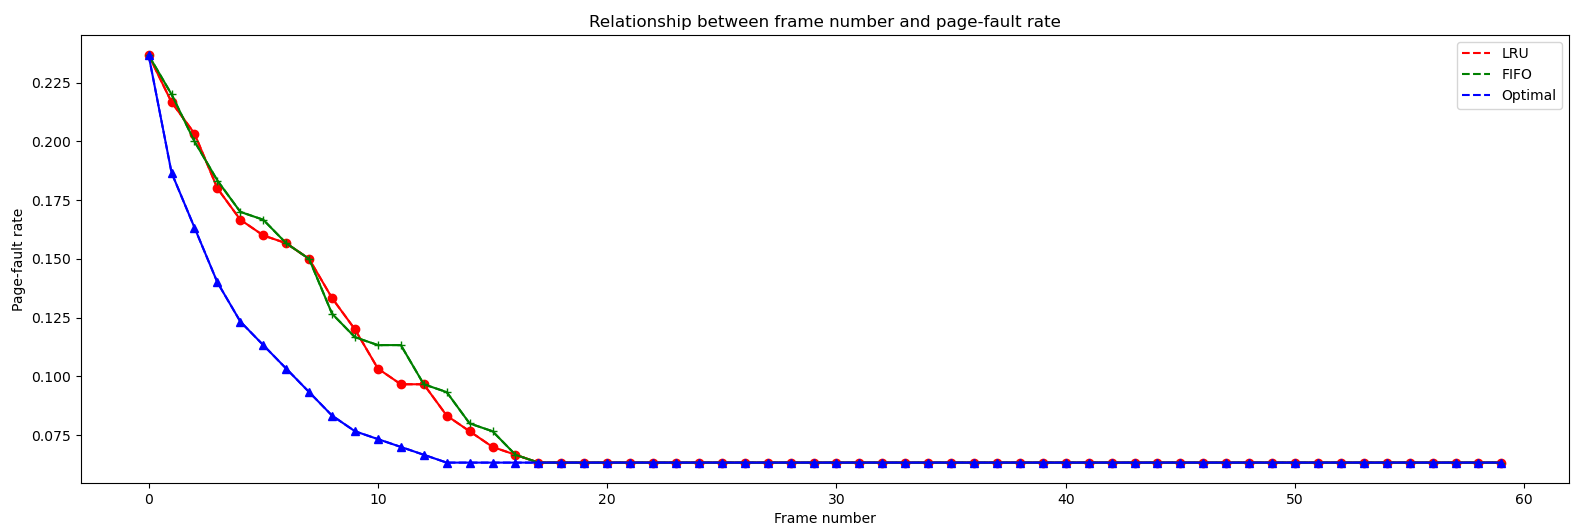
\includegraphics[width=\textwidth]{./images/Figure_2.png}
    \caption{\label{fig:2}}

\end{figure}

可以发现随着页表大小的增加,缺页率都呈下降趋势,最优置换算法的下降最快,LRU次之,FIFO最慢。

\section{实验总结}

本次实验中我实现了三种页面置换算法,并且对它们的性能进行比较,使我对相关知识点的掌握更加牢固。

实验结果显示最优页面置换算法的优异性能,然而LRU算法的性能却和FIFO算法接近,这是由于数据生成的过程没有考虑页面访问的局部性所致,数据的随机生成仍然有优化空间。

本次实验使我的C编程能力得到提高,我从中收获颇丰。

\end{document}